%%%%%%%%%% 3D PRINTER %%%%%%%%%%%%%%%%%%%%%%%%%%%%%%%%%%%%%%%%%%%%%%%%%%%%%
\subsection{3D Printer}

	3D printers are Computer Numerical Control (CNC) machines that are capable of transforming virtual 3D models created with a Computer Aided Design (CAD) software into real-world objects.\\

	Created in 1984 by Chuck Hull of 3D Systems Corp this technology was little-known to the general public and was mainly used in industries for short runs of difficult pieces.\\
	In 2005 Dr. Adrian Bowyer, from the University of Bath, UK, started the RepRap project. Its goal was "to produce a pure self-replicating device not for its own sake, but rather to put in the hands of individuals anywhere on the planet, for a minimal outlay of capital, a desktop manufacturing system that would enable the individual to manufacture many of the artifacts used in everyday life" \\

	Today a vast range of 3D printers co-exist, varying in size, price and materials used. \\


	$\rightarrow$ [RepRap, Zcorp, chocolate, liquid sint, micro, house building]\\

	$\rightarrow$ [table with different methods?]\\

	In this theses a RepRap Prusa Air 2 designed by Manuel Palacios is used. It is of a "fused filament fabrication additive manufacturing" type. This type of printers extrude mainly ABS or PLA plastics, and deposit new liquified material over ther previous layer, now solid, effectively building parts from the bottom up layer by layer.

	$\rightarrow$ \textbf {Terminal Imprusión Autorreplicante (T.I.A) }
	(add info + pic)
	Built within the scope of the Clone Wars project



%%%%%%%%%% 3D SOFTWARE %%%%%%%%%%%%%%%%%%%%%%%%%%%%%%%%%%%%%%%%%%%%%%%%%%%%
\subsection{Software}
	3D printers work by turning 3D models into plastic parts. These models are first modelled in a CAD program and then processed with a \textit{slicing} software to divide the model into layers of G-code, which is the standard language interpreted by CNCs. This is then introduced in a third piece of software which feeds it to the printer.

		\subsubsection{3D Modelling }
		In this project Sketchup has been used to create the printed parts. Owned by the company Trimble Navigation it is a WYSIWYG (What You See Is What You Get) modelling editor with a large online warehouse of parts available for download. \\

			\begin{figure}[H]
				\centering
				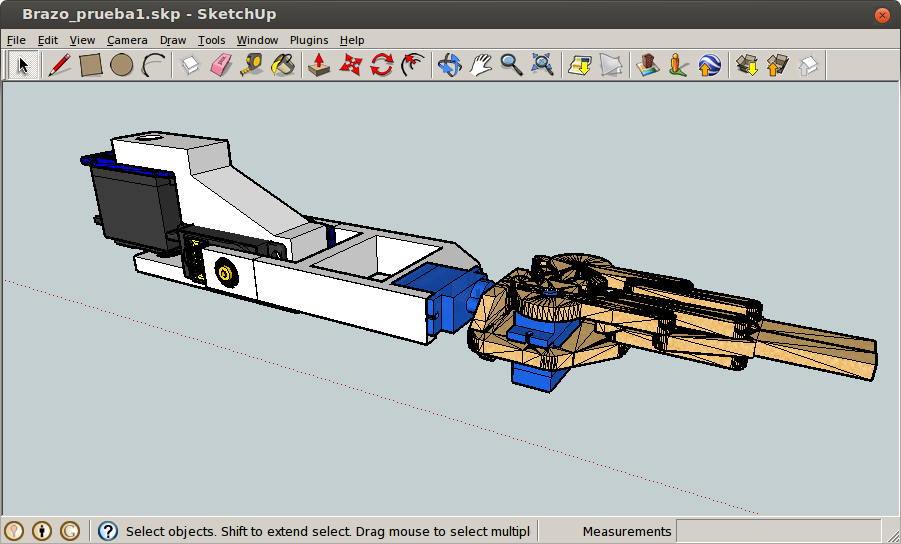
\includegraphics[scale=0.4]{images/ProjectComponents/sketchup-arm.png}
				\caption{SketchUp software}
				\label{}
			\end{figure}
			\bigskip

		In order to make it compatible with the slicing sofware, Sketchup's propietary format, \textit{SKP}, has to be converted to the standard \textit{STL}. In order to accomplish this the \textit{Su2stl.rb} plugin is installed. A new \textit{Plugins} menu appears in Sketchup which contains the Import/Export options, where the desired output format and model units are specified.



		\subsubsection{G-Code Generator} 
		Once the model is converted to \textit{STL} it then has to be sliced. Since 3D printers work by building layer upon layer of plastic, the model has to be transformed into the same format. The G-code generator converts the CAD model into layers of CNC instructions. There are three main slicing programs, each with their own benefits:

			\begin{itemize}
			  
			  \item Skeinforge: \hfill \\
			  The first slicing program used in homemade 3D printers. It is by far the most complete of the three. It allows the user to control each and every imaginable setting of the printer, from the axis' speeds to the retraction distance of the plastic into the extruder while moving. However, because of this it has a very steep learning curve which makes it unsuitable for the average consumer.

			  \item Slic3r:  \hfill \\
			  Slic3r was created as an user-friendly software, which only gives the final user a choice in the basic settings, such as printing speeds, filament widths or part infills. As a result it is an easier program to slice parts with a sufficient level of customization. It has nonetheless problems converting models with imperfections or broken shapes.
			  
			  \item Cura \hfill \\
			  Finally, Cura is also designed with user-friendliness in mind. This slicer is more robust than Slic3r, in that it will accept models with imperfections, and will try to correct them. It also features a box simulating the print area in which the model can be moved around, turned or scaled before printing.
			  This last feature is specially useful if minor changes need to be made, without returning to the CAD software.
			
			\end{itemize}



		\subsubsection{CNC Controller}


%%%%%%%%%%%% BATTERY %%%%%%%%%%%%%%%%%%%%%%%%%%%%%%%%%%%%%%%%%%%%%%%%%%%%%%
\subsection{Li-Ion Battery}

	The whole system is powered by a lithium ion 12V 6800mAh battery. 

		\begin{figure}[H]
				\centering
				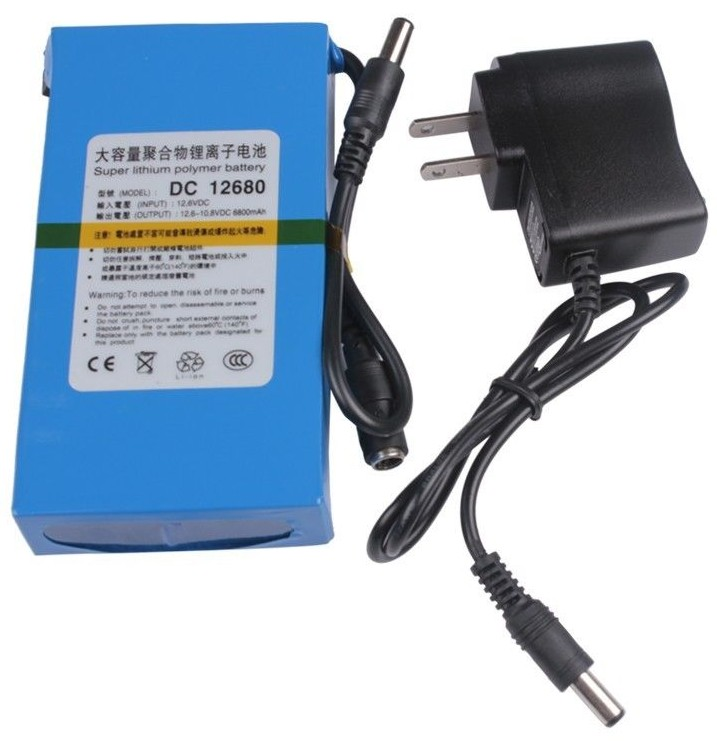
\includegraphics[scale=0.25]{images/ProjectComponents/battery.jpg}
				\caption{Li-ion 12V 6800mAh battery with charger}
				\label{}
		\end{figure}
		\bigskip

		\begin{figure}[H]
				\centering
				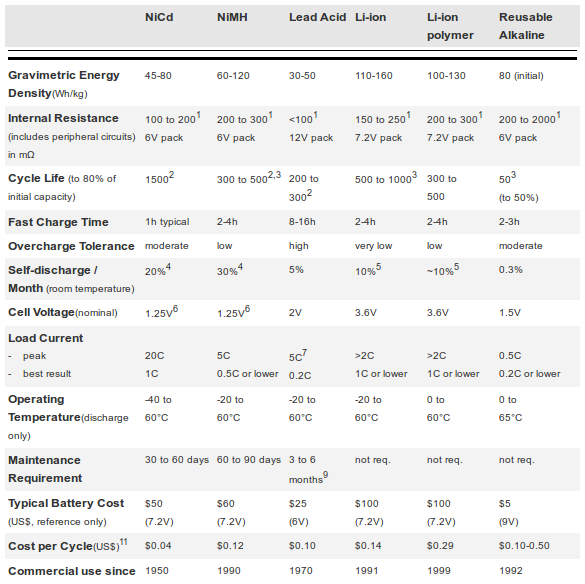
\includegraphics[scale=0.75]{images/ProjectComponents/battery-differences.png}
				\caption{Table comparing different battery technologies}
				\label{}
		\end{figure}
		\bigskip

%%%%%%%%%%% CONVERTER %%%%%%%%%%%%%%%%%%%%%%%%%%%%%%%%%%%%%%%%%%%%%%%%%%%%%
\newpage
\subsection{Voltage level converters}	
	
	\subsubsection{DC-DC Step-Down Converter}

		This DC-DC voltage conveter is used to decrease the battery's voltage from 12V to the 5V required by the logic components as well as the servomotors.

			\begin{figure}[H]
					\centering
					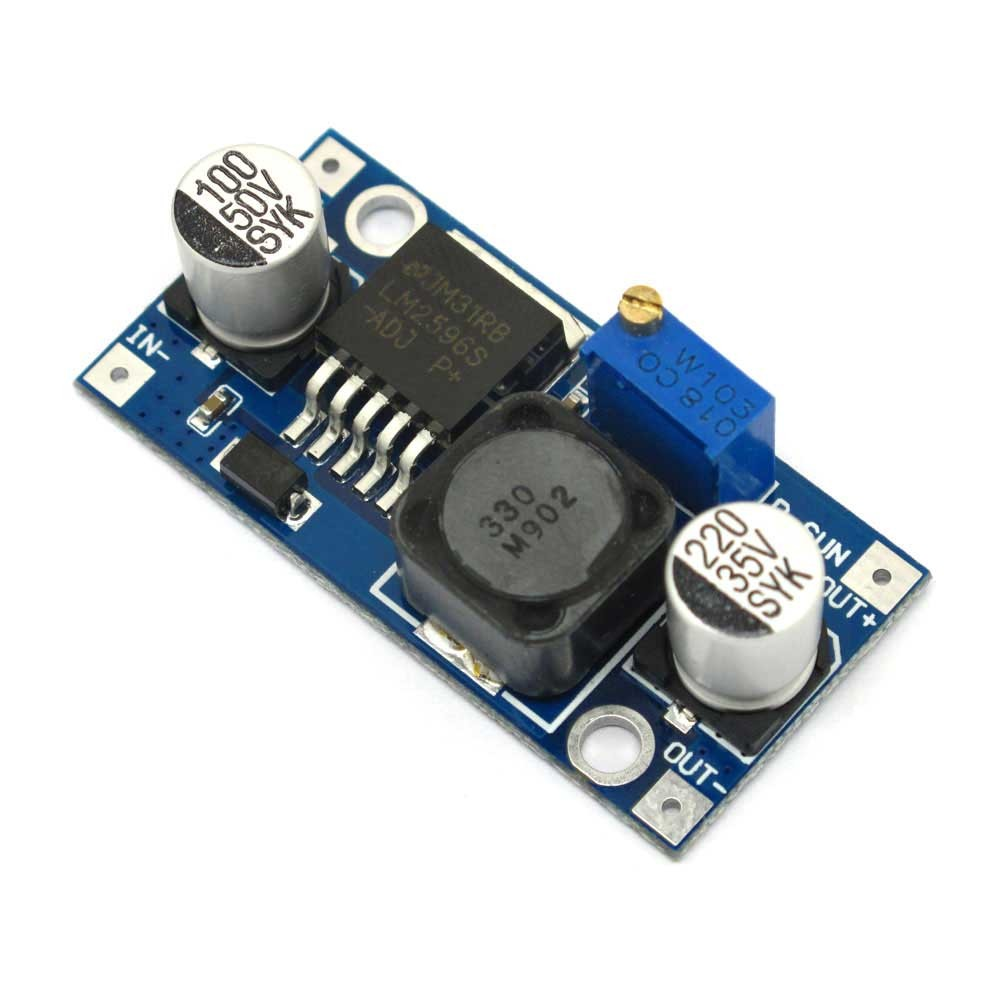
\includegraphics[scale=0.2]{images/ProjectComponents/buck.jpg}
					\caption{Step-down converter }
					\label{}
			\end{figure}
			\bigskip

		The converter's electrical specifications are:
			\begin{itemize}
				\item Adjustable input voltage: 3.2 - 40V
				\item Adjustable output voltage: 1.25 - 35V (require input voltage 1.5V high than output voltage)
				\item Max. output current: 3A
			\end{itemize}

	\subsubsection{Bi-directional logic level converter}

		This logic level converter is used to enable serial communication between the Arduino and the Raspberry Pi, since the latter's 3.3V operation point could be damaged by the former's 5V high-level. 

			\begin{figure}[H]
					\centering
					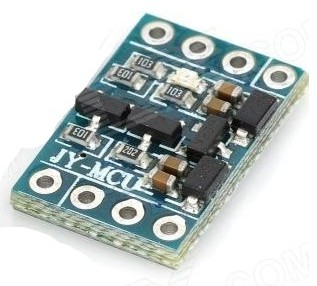
\includegraphics[scale=0.4]{images/ProjectComponents/logic-voltage.jpg}
					\caption{Bi-directional logic level converter }
					\label{}
			\end{figure}
			\bigskip

		This board is used with UART communication, but is equally adequate for I$^2$C, SPI or even one-wire communication.
 
%%%%%%%%%%% DC MOTORS %%%%%%%%%%%%%%%%%%%%%%%%%%%%%%%%%%%%%%%%%%%%%%%%%%%%%
\subsection{Motors}

	\subsubsection{GA25Y370 DC motor}
	
		\begin{figure}[H]
			\centering
			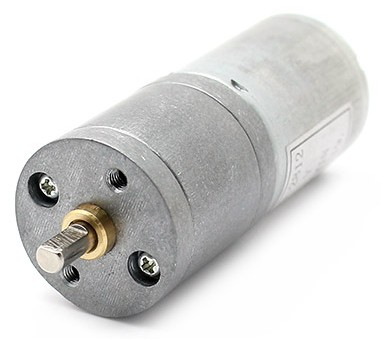
\includegraphics[scale=0.4]{images/ProjectComponents/motor.jpg}
			\caption{GA25Y370 motor }
			\label{}
	\end{figure}
	\bigskip

	\subsubsection{GOTECK GS-551MG servomotor}

		\begin{figure}[H]
			\centering
			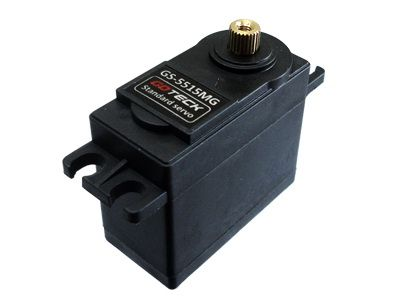
\includegraphics[scale=0.5]{images/ProjectComponents/servo1.jpg}
			\caption{GOTECK GS-551MG servo }
			\label{}
	\end{figure}
	\bigskip


	\subsubsection{TowerPro SG90 servomotor}

		\begin{figure}[H]
			\centering
			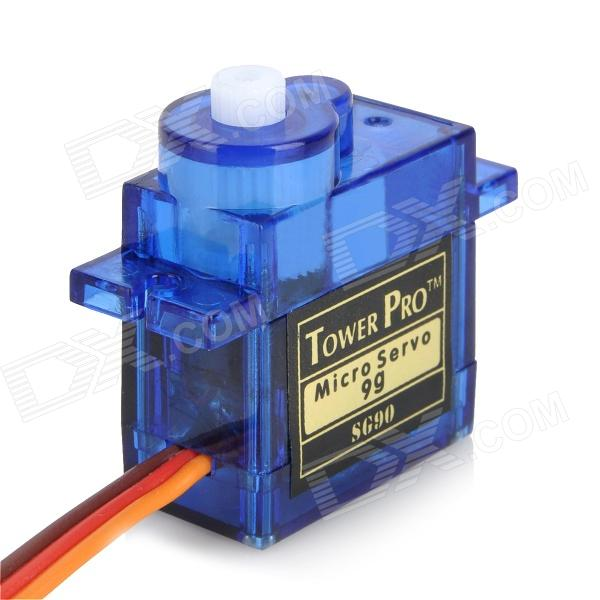
\includegraphics[scale=0.25]{images/ProjectComponents/servo2.jpg}
			\caption{TowerPro SG90 servo }
			\label{}
	\end{figure}
	\bigskip





%%%%%%%%%%%% ARDUINO %%%%%%%%%%%%%%%%%%%%%%%%%%%%%%%%%%%%%%%%%%%%%%%%%%%%%%
\newpage
\subsection{Arduino}

	Arduino is a family of low-cost electronic boards designed to be easily programmable. From the official Arduino website, "Arduino is an open-source electronics prototyping platform based on flexible, easy-to-use hardware and software. "\\

	Arduino is programmed using its own language, which is merely a set of C/C++ functions compiled with \textit{avr-g++}. They can nonetheless be programmed in pure C or C++ in an external IDE and have code uploaded as any other AVR board.\\

	In this proyect an Arduino Nano v3 with an ATmega 328 microcontroller has been chosen mainly due to its processing power and reduced size.
		
		\begin{figure}[H]
			\centering
			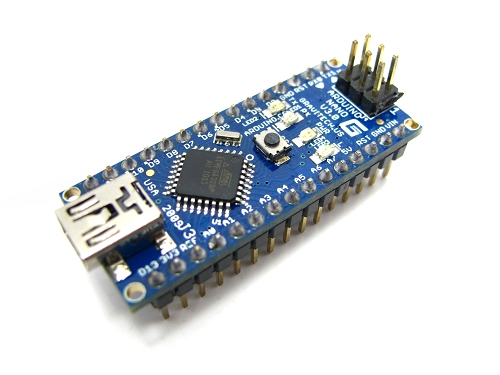
\includegraphics[scale=0.4]{images/ProjectComponents/arduino.jpg}
			\caption{Arduino Nano v3 }
			\label{}
		\end{figure}
		\bigskip

	The official Arduino Nano V3 specifications are:
		\begin{itemize}
			\item \textbf{Microcontroller:} Atmel ATmega168 or ATmega 328
			\item \textbf{Operating Voltage (logic level):} 5V
			\item \textbf{Input Voltage (recommended):} 7-12V
			\item \textbf{Input Voltage (limits):} 6-20V
			\item \textbf{Digital I/O Pins:} 14 (of which 6 provide PWM output)
			\item \textbf{Analog Input Pins:} 8
			\item \textbf{DC Current per I/O Pin:} 40mA
			\item \textbf{Flash Memory:} 16 KB (ATmega168) or 32 KB (ATmega328), of which 2 KB used by bootloader
			\item \textbf{SRAM:} 1 KB (ATmega168) or 2 KB (ATmega328)
			\item \textbf{EEPROM:} 512 bytes (ATmega168) or 1 KB (ATmega328)
			\item \textbf{Clock Speed:} 16MHz
			\item \textbf{Dimensions:} 0.73'' x 1.70''
			\item \textbf{Communications:} UART, SPI and I$^2$C buses
		\end{itemize}



%%%%%%%%%%% RASPBERRY %%%%%%%%%%%%%%%%%%%%%%%%%%%%%%%%%%%%%%%%%%%%%%%%%%%%%
\newpage
\subsection{Raspberry Pi}

	From the official website of the homonymous foundation, the Raspberry Pi is a "credit-card sized computer that plugs into your TV and a keyboard. It is a capable little computer which can be used in electronics projects."\\

		\begin{figure}[H]
				\centering
				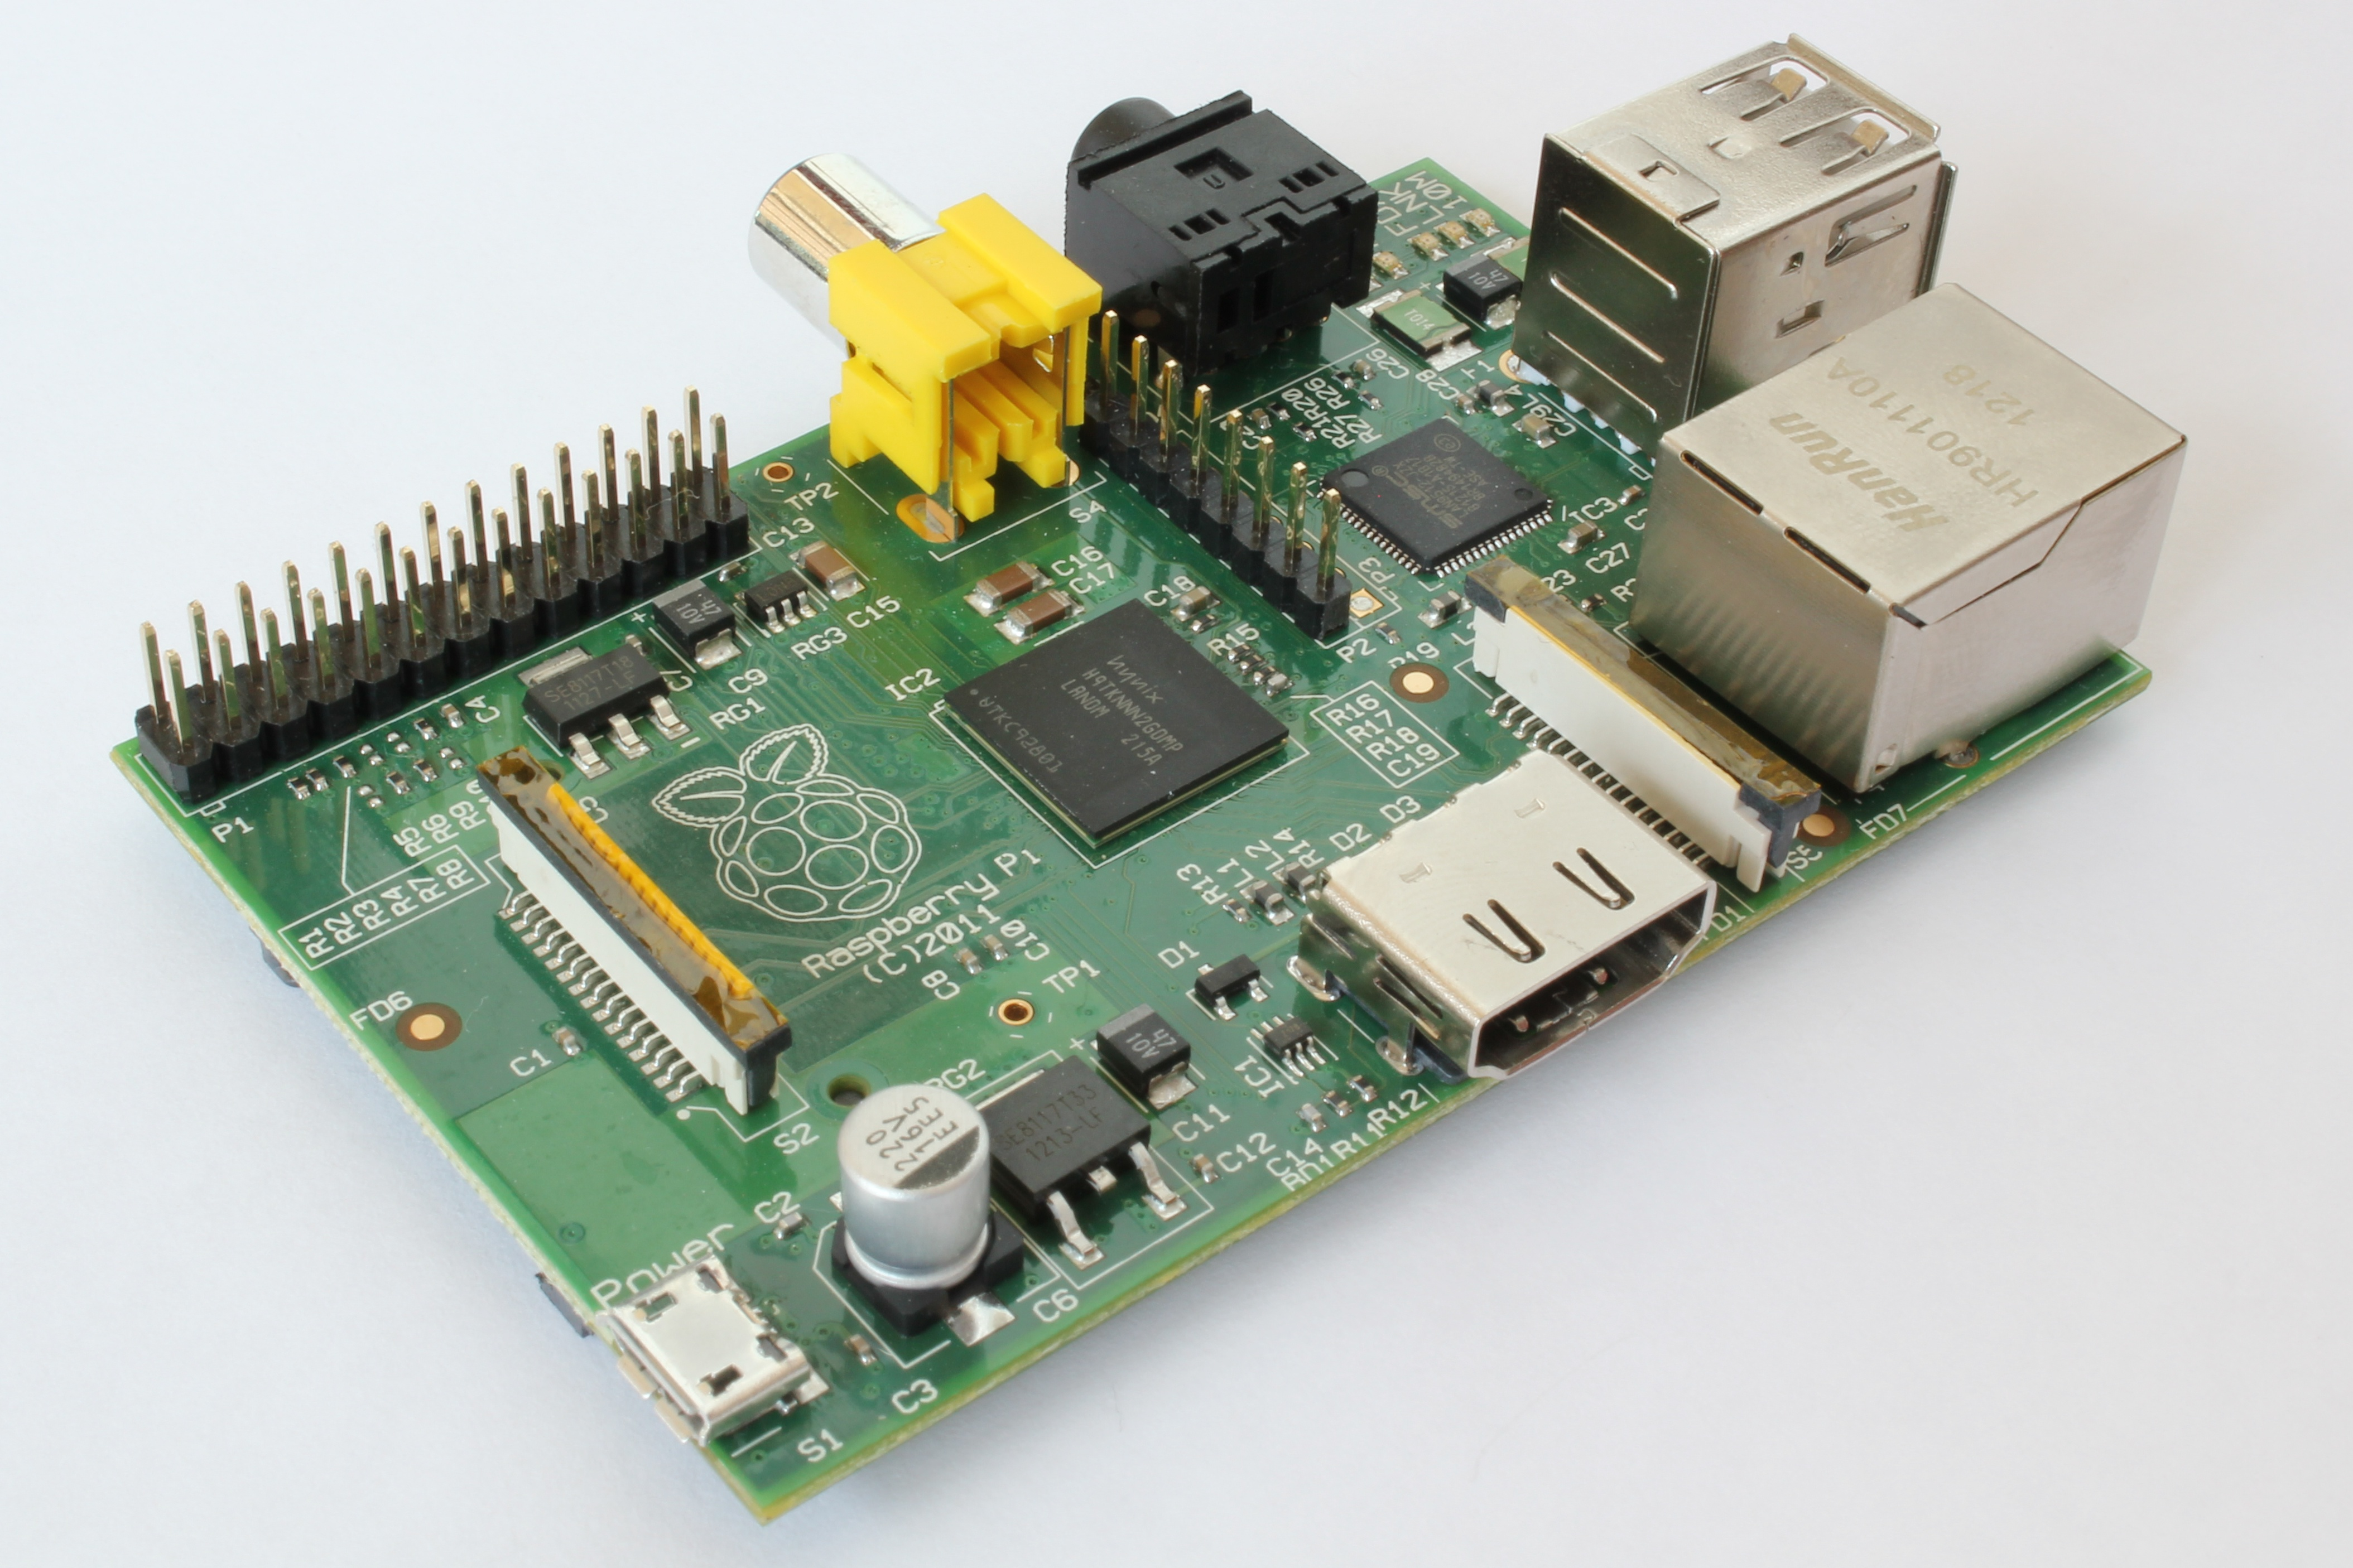
\includegraphics[scale=0.07]{images/ProjectComponents/raspberry.jpg}
				\caption{Raspberry Pi model B}
				\label{}
		\end{figure}
		\bigskip

	Available in two models, A and B, the Raspberry has a Broadcom BCM2835 System On a Chip, which includes an ARM1176JZF-S 700MHz processor and a VideoCore IV GPU. It includes as well a 256Mb RAM, upgraded to 512Mb in model B.\\

	\bigskip

	The Pi features: 
		\begin{itemize}
			  \item HDMI, composite and raw DSI video outputs
			  \item 3.5mm audio jack
			  \item SD card socket
			  \item Low-level peripheral connections including:
			  	\begin{itemize}
			  	\item 8 General Purpose Input Output (GPIO) pins
			  	\item Universal Asynchronous Receiver Transmitter (UART) bus
			  	\item Inter-Integrated Circuit (I$^2$C) bus
			  	\item 2 Serial Peripheral Interface (SPI) buses
			  	\item Power pins: 3.3V, 5V and GND
			  	\end{itemize}
			  \item Ethernet socket
			  \item USB hub (1 socket in model A, 2 in model B)

		\end{itemize}

	The main storage unit is the SD card, and that is where the OS is flashed, normally a Linux distribution. The most popular is Raspbian, an adapted version of Debian Wheezy, although other Linux distros or even other OS like Android or XBMC can be used.

		\begin{figure}[H]
		    \centering
		    \begin{subfigure}[b]{0.3\textwidth}
		        \centering
		        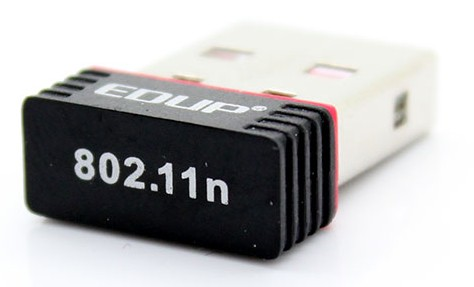
\includegraphics[scale=0.25]{images/ProjectComponents/wifi.jpg}
				\caption{WiFi USB dongle}
		        \label{}
		    \end{subfigure}
		    \hfill
		    \begin{subfigure}[b]{0.3\textwidth}
		        \centering
		        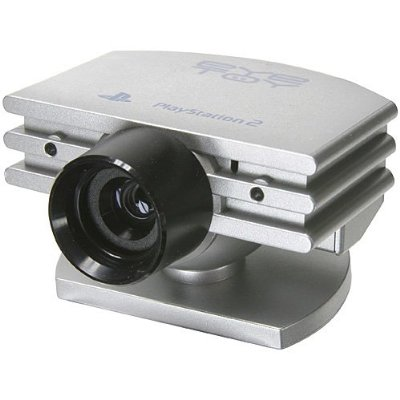
\includegraphics[scale=0.25]{images/ProjectComponents/camera.jpg}
				\caption{PlayStation 2 EyeToy }
		        \label{}
		    \end{subfigure}
		    \hfill
		    \begin{subfigure}[b]{0.3\textwidth}
		        \centering
		      	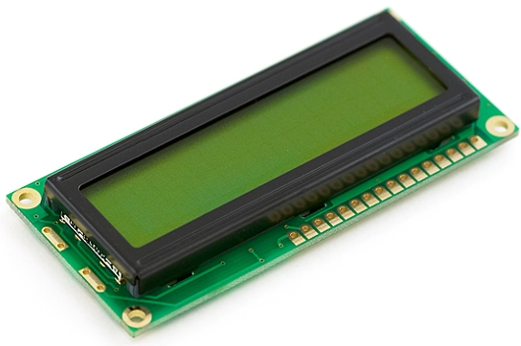
\includegraphics[scale=0.25]{images/ProjectComponents/lcd.jpg}
				\caption{LCD screen 16x2}
		        \label{}
		    \end{subfigure}
		    \caption{Raspberry Pi peripherals}
		    \label{}
		\end{figure}


	In this proyect a Raspberry Pi model B running Raspbian manages the software side of the robot. It has an EDUP 802.11n WiFi USB dongle , a PlayStation 2 EyeToy USB camera and a 16x2 character LCD screen connected in order to create a WIFI Access Point, stream video to the user and signal its status respectively.



% %%%%%%%%%%% LCD SCREEN %%%%%%%%%%%%%%%%%%%%%%%%%%%%%%%%%%%%%%%%%%%%%%%%%%%%
% \subsection{LCD Screen}

% 	\begin{figure}[H]
% 			\centering
% 			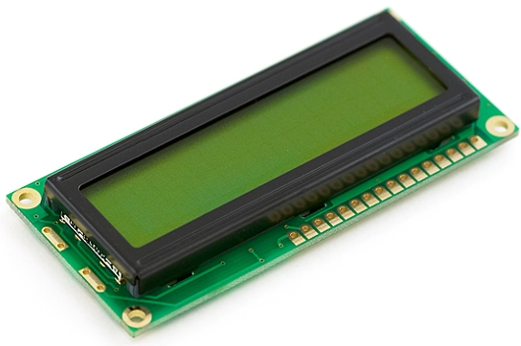
\includegraphics[scale=0.4]{images/ProjectComponents/lcd.jpg}
% 			\caption{LCD screen 16x2}
% 			\label{}
% 	\end{figure}
% 	\bigskip

% %%%%%%%%%%% WIFI USB %%%%%%%%%%%%%%%%%%%%%%%%%%%%%%%%%%%%%%%%%%%%%%%%%%%%%%
% \subsection{WiFi USB}

% 	\begin{figure}[H]
% 			\centering
% 			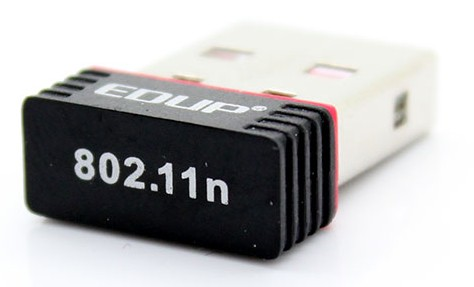
\includegraphics[scale=0.4]{images/ProjectComponents/wifi.jpg}
% 			\caption{WiFi USB dongle}
% 			\label{}
% 	\end{figure}
% 	\bigskip

% %%%%%%%%%%% CAMERA %%%%%%%%%%%%%%%%%%%%%%%%%%%%%%%%%%%%%%%%%%%%%%%%%%%%%%%%
% \subsection{Camera}

% 	\begin{figure}[H]
% 			\centering
% 			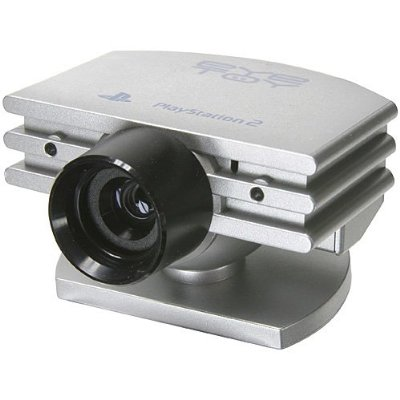
\includegraphics[scale=0.4]{images/ProjectComponents/camera.jpg}
% 			\caption{PlayStation 2 EyeToy camera }
% 			\label{}
% 	\end{figure}
% 	\bigskip






%%%%%%%%%%% ANDROID %%%%%%%%%%%%%%%%%%%%%%%%%%%%%%%%%%%%%%%%%%%%%%%%%%%%%%%
\newpage
\subsection{Android Phone}

	\begin{figure}[H]
			\centering
			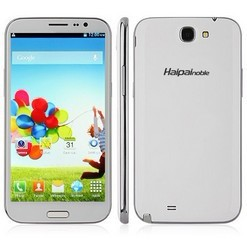
\includegraphics[scale=0.8]{images/ProjectComponents/android.jpg}
			\caption{Android smartphone Haipai Noble H868}
			\label{}
	\end{figure}
	\bigskip

